%\documentclass[envcountsect,11pt,trans]{beamer}
\documentclass[11pt,aspectratio=169]{beamer}
\usepackage[english]{babel}
\usepackage[ansinew]{inputenc}
\usepackage{times}
\usepackage{xcolor}
\usepackage{graphicx}
\usepackage{rotating}
\usepackage{bbding,pifont} % two dingbat fonts
\usepackage{amsmath}
\usepackage{amsfonts}
\usepackage{amssymb}
\usepackage{fancybox}
\usepackage{epstopdf}
\usepackage{eso-pic}
%\usepackage[round]{natbib}
\usepackage{ngerman}
\usepackage{tcolorbox}
\usepackage{colortbl}
%\usepackage[authordate,bibencoding=auto,strict,backend=biber]{biblatex-chicago}
%\usepackage{natbib}
%\usepackage[style=bath, backend=biber]{biblatex}
\usepackage{ulem}
\usepackage{tikz}
\usepackage{booktabs}
\usepackage{longtable}
\usepackage{hyperref}
\usepackage{array}
\usepackage{appendixnumberbeamer}
\usepackage[T1]{fontenc}
\usepackage{adjustbox}
\usepackage{listings}
\usepackage{uarial}
\usepackage{fancyvrb}
\usepackage{subfigure}
\renewcommand{\familydefault}{\sfdefault}

\newcommand*\circled[1]{\tikz[baseline=(char.base)]{
            \node[shape=circle,draw,inner sep=2pt] (char) {#1};}}
\newcommand{\E}{\operatorname{E}}
\newcommand{\Var}{\operatorname{Var}}
\newcommand{\overbar}[1]{\mkern 1.5mu\overline{\mkern-1.5mu#1\mkern-1.5mu}\mkern 1.5mu}
\DeclareMathOperator*{\argmin}{arg\,min}
\DeclareMathOperator*{\argmax}{arg\,max}
% \use\smallpackage{pgfpages}
% \pgfpagesuselayout{4 on 1}[a4paper,border shrink=10mm,landscape]

%\xdefinecolor{MyColor}{rgb}{0.14,0.17,0.52}
%\xdefinecolor{MyColor}{rgb}{0.29,0.53,0.82}
%\xdefinecolor{MyBlue}{rgb}{0.14,0.17,0.52}
%\xdefinecolor{MyGreen}{rgb}{0.70,0.78,0.14}
%\xdefinecolor{MyAlert}{rgb}{0.29,0.53,0.82}
%\colorlet{mystructure}{MyColor}
%\usecolortheme[named=mystructure]{structure}
%\setbeamercolor{alerted text}{fg=MyAlert}
\definecolor{Black}{RGB}{0,0,0}
\definecolor{RedGIZ}{RGB}{200,15,15}
\setbeamercolor{title}{fg=black}
\setbeamercolor{section in toc}{fg=black}
\setbeamercolor{subsection in toc}{fg=black}
\setbeamercolor{frametitle}{fg=Black}
\setbeamercolor{tableofcontents}{fg=Black}

%\usetheme{Boadilla}
%\usetheme{Madrid}
%\useoutertheme{infolines}
%\usecolortheme{whale}
%\usecolortheme{lily}
\renewcommand{\inserttitlegraphic}{
\parbox[b][2.5cm][t]{4cm}{
\includegraphics[width = 4cm, keepaspectratio]{pictures/GIZ_Logo.png}}  \hspace{0.1cm} \parbox[b][2.5cm][t]{4cm}{
\includegraphics[width = 4cm, keepaspectratio]{pictures/IWH_Logo_RGB_DE_Grossformat.png}} \hfill \parbox[b][2.5cm][t]{3.21cm}{
\includegraphics[keepaspectratio,width=4.00cm]{pictures/seperationbar.png} \\ \includegraphics[width = 4cm, keepaspectratio]{pictures/BMWI_logo.png}}
}
\defbeamertemplate*{title page}{customized}[1][]
{	
	\vspace{2.75cm}
  \usebeamerfont{title}\begin{center}\textbf{\inserttitle}\end{center}\par
  \usebeamerfont{subtitle}\begin{center}\usebeamercolor[fg]{subtitle}\insertsubtitle\end{center}\par
  \usebeamerfont{author}\insertauthor $\, \vert$ \usebeamerfont{date}\insertdate \par
  \usebeamerfont{institute}\insertinstitute\par
	\vspace{0.25cm}
  \usebeamercolor[fg]{titlegraphic}\inserttitlegraphic


}
\setbeamerfont{subtitle}{size=\normalsize}
\setbeamerfont{author}{size=\tiny}
\setbeamerfont{date}{size=\tiny}
\setbeamerfont{institute}{size=\tiny}

\setbeamercovered{transparent}

\setbeamertemplate{footline}[text line]{%
  \parbox{\linewidth}{\vspace*{-8pt} $\vert$ \hspace{1mm} \today \hspace{1mm} $\vert$ \hfill}}
\setbeamertemplate{navigation symbols}{}

\linespread{1.2}





\mode<presentation>{
    \setbeamertemplate{itemize item}{\color{RedGIZ}$\blacksquare$}
    \setbeamertemplate{itemize subitem}{\color{RedGIZ}$\blacktriangleright$}
		}
\title[DGE--CRED]{Dynamic General Equilibrium Model for Climate Resilient Economic Development}
%\subtitle[]{Training}

\author[Christoph Schult]{Andrej Drygalla, Katja Heinisch and Christoph Schult*} \date[July 2020]{July 2020}
\institute[IWH]{Halle Institute for Economic Research}

 
\logo{\begin{tabular}{c}
\includegraphics[keepaspectratio,width=1.00cm]{pictures/seperationbar.png} \\ 
\includegraphics[keepaspectratio,width=1.00cm]{pictures/GIZ_Logo}\end{tabular}}

\usepackage[style=authoryear,maxbibnames=9,maxcitenames=2,backend=bibtex]{biblatex}
\bibliography{references}

% Settings by yw:
% Outline at beginning of each section:
\AtBeginSection[]{	
	{\setbeamertemplate{footline}{}
	\begin{frame}<beamer>{Outline}
		\tableofcontents[sectionstyle=show/hide, subsectionstyle=show/show/hide, subsubsectionstyle=show/show/hide]
		\setbeamertemplate{footline}{}
		\addtocounter{framenumber}{-1}
	\end{frame}}
}
% Packages:
\usepackage{ragged2e}
\usepackage{upquote}
\usepackage{subfigure}
\usepackage{ragged2e}
\lstset{ 
  backgroundcolor=\color{white},
	breaklines=true,
	basicstyle=\tiny
}
% Section numbering:
\setbeamertemplate{section in toc}[sections numbered]
\setbeamertemplate{subsection in toc}[subsections numbered]
\setbeamertemplate{subsubsection in toc}[subsubsections numbered]
\setbeamertemplate{section in toc}[ball]
\setbeamertemplate{subsection in toc}[ball]
\setbeamertemplate{subsubsection in toc}[ball]
\setbeamercolor{section number projected}{bg={RedGIZ}}
\setbeamercolor{subsection number projected}{bg={RedGIZ}}
\setbeamercolor{subsubsection number projected}{bg={RedGIZ}}
%\usefonttheme{serif}
\begin{document}
%\footnotesize
\usebackgroundtemplate{
\vbox to \paperheight{\vspace{0.1cm}\hbox to \paperwidth{\hfil
\includegraphics[width=0.975\paperwidth,height = 0.7\paperheight]{pictures/BackgroundGIZ.jpg}\hfil}\vfil
}}

\begin{frame}<presentation>[noframenumbering,plain]
  \titlepage \\
	{\tiny} \scalebox{.4}{* Research assistance by Yoshiki Wiskamp is greatly acknowledged.}
\end{frame}
\usebackgroundtemplate{
}
{\setbeamertemplate{footline}{}
\begin{frame}<presentation>[noframenumbering]
	\frametitle{Outline}
		 \tableofcontents[hideallsubsections]
\end{frame}
}
%%%%%%%%%%%%%%%%%%%%%%%%%%%%%%%%%%%%%%%%%%%%%%%%%%%%%%%%

\section{DGE-CRED Model: Scenario Creation and Simulation}

\subsection{Introduction}

\begin{frame}<presentation>
\frametitle{{\thesection.\thesubsection} Introduction}
	\begin{itemize}
		\item The DGE-CRED model allows its user to analyze and compare different \textit{scenarios}
		\begin{itemize}
			\item The model can be used without a detailed knowledge about programming 
			\item The user has to edit an excel sheet in order to: (i) set the paths of the exogenous variables, (ii) specify the initial and terminal values, (iii) assign parameter values, etc.
		\end{itemize}
		\item The following slides encompass a guideline on how to \textit{create} and \textit{simulate} a new \textit{scenario} 
		\begin{itemize}
			\item For a comprehensive explanation on how to set the structural parameters for the simulation, see the presentation ``DGE\_CRED\_Training''
		\end{itemize}
	\end{itemize}
\end{frame}

\subsection{\texttt{ModelSimulationandCalibration\textcolor{red}{k}Sectorsand\textcolor{red}{r}Regions.xlsx}}

\begin{frame}<presentation>
\frametitle{{\thesection.\thesubsection} Setting up a new Sceanrio (1)}
	\begin{itemize}
			\item At first, the user has to choose the:
				\begin{itemize}
					\item number of sectors \textcolor{red}{k}
					\item number of regions \textcolor{red}{r}
				\end{itemize}
			\item The settings for the simulation of \textcolor{red}{k} sectors and \textcolor{red}{r} regions must be provided in ``\texttt{ModelSimulationandCalibration\textcolor{red}{k}Sectorsand\textcolor{red}{r}Regions.xlsx}''
			\item To create a new \textit{scenario}, a new sheet has to be added to this workbook
			\begin{itemize}
				\item The name of the sheet becomes the name of the scenario
				\item Avoid using symbols or spaces when naming the scenario
				\item Examples of valid scenario names: \texttt{RCP\_45\_Average}, \texttt{Baseline}
			\end{itemize}
	\end{itemize}
\end{frame}
\begin{frame}<presentation>
	\frametitle{{\thesection.\thesubsection} Setting up a new Sceanrio (2)}
	\begin{itemize}
		\item The trajectories of the \textit{exogenous} variables examined in this new scenario must be added to the excel sheet
		\begin{itemize}
			\item As the initial value is provided in the sheet ``\texttt{start}'', values starting from period $t=2$ must be provided
			\item Note that absolute changes compared to the initial value must be provided
			\item If no specific trajectory for an exogenous variable is provided in this sheet, the variable will remain at its initial value 
			\item Include a timeline in the first column of the sheet
			\item Recommendation: Include a trajectory for population (\texttt{exo\_PoP})
		\end{itemize}
	\end{itemize}
\end{frame}
\begin{frame}<presentation>
	\frametitle{{\thesection.\thesubsection} Setting up a new Sceanrio (3)}
	\begin{itemize}
		\item Example: Set up a new scenario called ``RCP\_45\_Average'' in a 3 sector and 3 regions setting. Include the trajectories of population (\texttt{exo\_PoP}), temperature (\texttt{exo\_T\_r}), precipitation (\texttt{exo\_PREC\_r}) and sea level (\texttt{exo\_SL}).
		\begin{figure}
			\frame{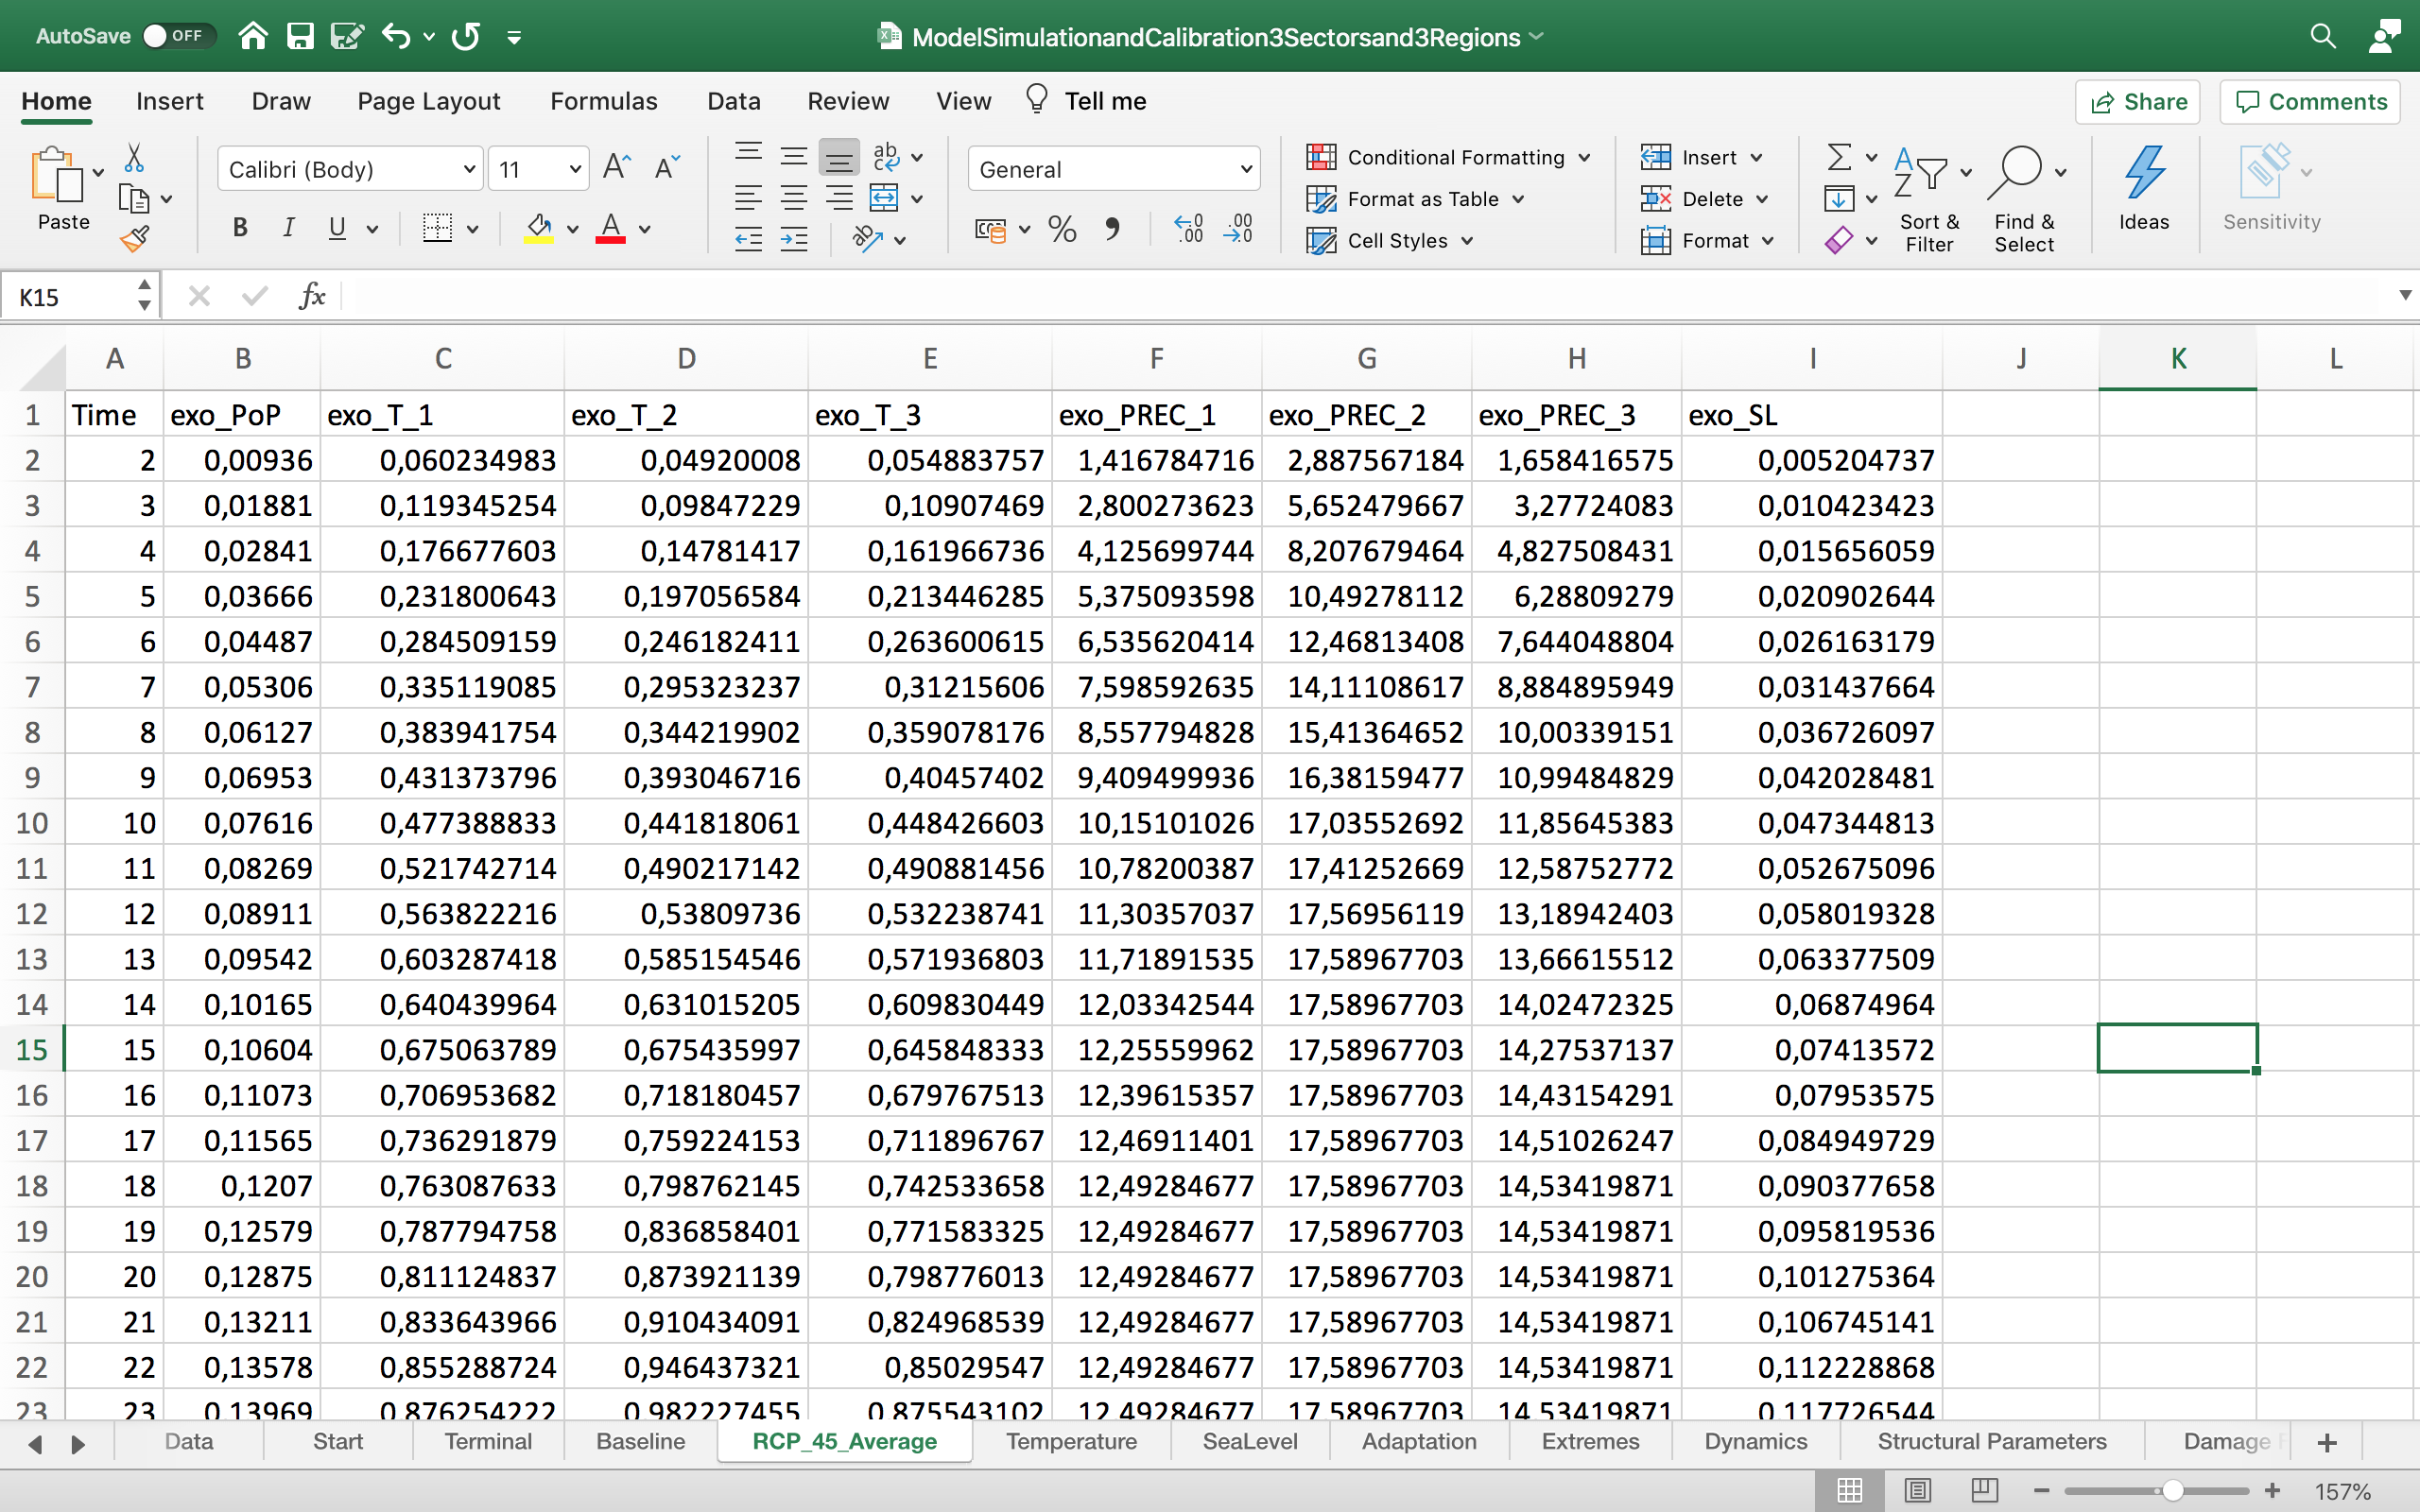
\includegraphics[width=8cm]{pictures/Scenario_Simulation/scensim01}}
		\end{figure}
	\end{itemize}
\end{frame}

\subsection{\texttt{DGE\_CRED\_Model.mod}}

\begin{frame}<presentation>
	\frametitle{{\thesection.\thesubsection} \texttt{DGE\_CRED\_Model.mod}}
	\begin{itemize}
		\item After creating a new scenario in ``\texttt{ModelSimulationandCalibration\textcolor{red}{k}Sectorsand\textcolor{red}{r}Regions.xlsx}'', open the Dynare file ``\texttt{DGE\_CRED\_Model.mod}''
		\item Define the number of sectors \textcolor{red}{k} and regions \textcolor{red}{r}
		\item Example:
		\begin{figure}
			\frame{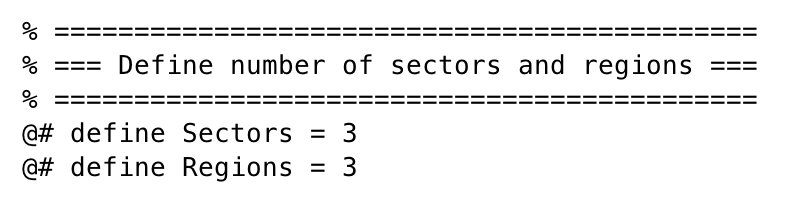
\includegraphics[width=7cm]{pictures/Scenario_Simulation/scensim02}}
		\end{figure}
	\end{itemize}
\end{frame}

\subsection{\texttt{RunSimulations.m}}

\begin{frame}<presentation>
	\frametitle{{\thesection.\thesubsection} \texttt{RunSimulations.m}}
	\begin{itemize}
		\item The next step is to open the MATLAB file ``\texttt{RunSimulations.m}'' and to specify the scenario names in ``\texttt{casScenarioNames}''
		\item Example:
		\begin{figure}
			\frame{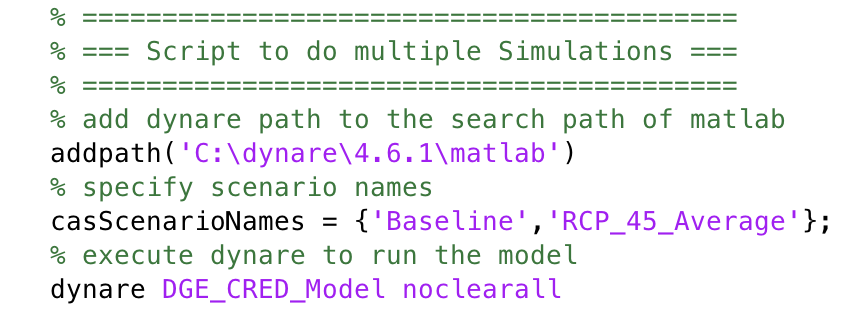
\includegraphics[width=7cm]{pictures/Scenario_Simulation/scensim03}}
		\end{figure}
		\item Now, everything is set up for the simulation of the new scenario
		\begin{itemize}
			\item Press ``Run'' to conduct the simulation
		\end{itemize}
	\end{itemize}
\end{frame}

\subsection{\texttt{ResultsScenarios\textcolor{red}{k}Sectorsand\textcolor{red}{r}Regions.xlsx}}

\begin{frame}<presentation>
	\frametitle{{\thesection.\thesubsection} \texttt{ResultsScenarios\textcolor{red}{k}Sectorsand\textcolor{red}{r}Regions.xlsx} (1)}
	\begin{itemize}
		\item The results of the simulation are stored in ``\texttt{ResultsScenarios\textcolor{red}{k}Sectorsand\textcolor{red}{r}Regions.xlsx}''
		\item There will be a result sheet for every scenario containing the trajectories of all model variables
	\end{itemize}
\end{frame}
\begin{frame}<presentation>
	\frametitle{{\thesection.\thesubsection} \texttt{ResultsScenarios\textcolor{red}{k}Sectorsand\textcolor{red}{r}Regions.xlsx} (2)}
	\begin{itemize}
		\item Example:
		\begin{figure}
			\frame{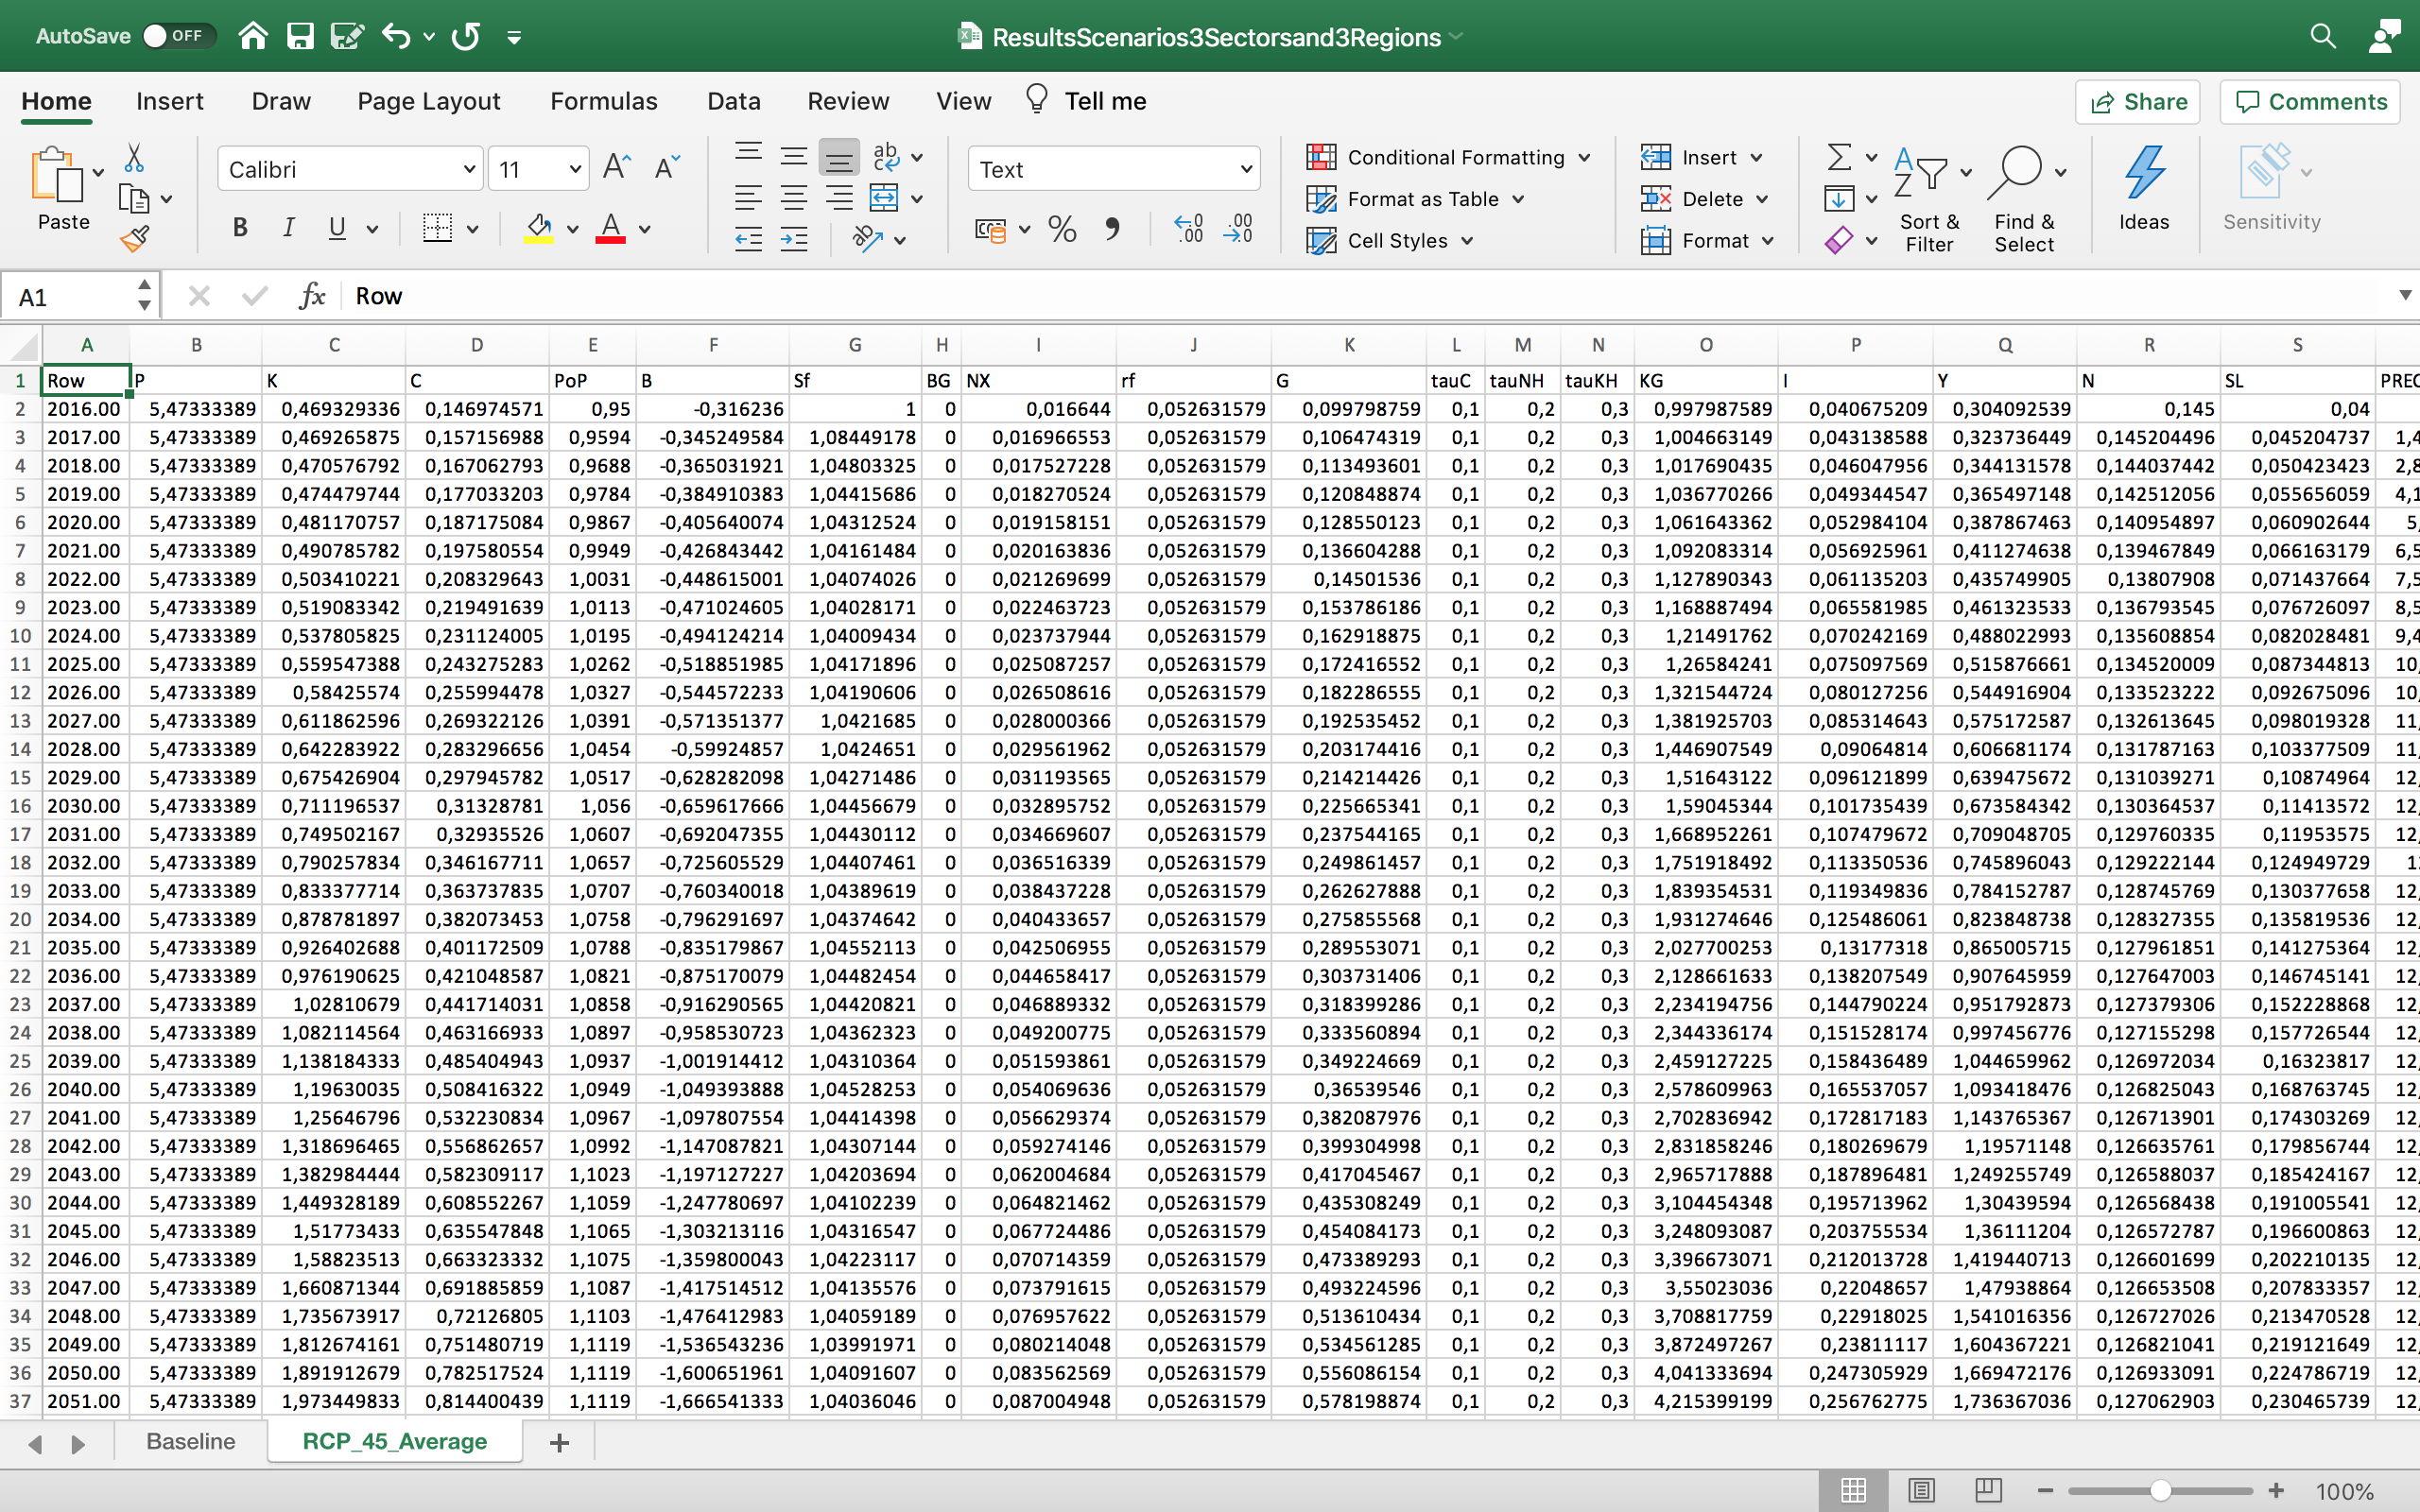
\includegraphics[width=8cm]{pictures/Scenario_Simulation/scensim04}}
		\end{figure}
	\end{itemize}
\end{frame}

\section{Appendix}

\subsection{Determine the Trajectories of the Climate Variables}

\begin{frame}<presentation>
	\frametitle{{\thesection.\thesubsection} Determine the Trajectories of the Climate Variables (1)}
	\begin{itemize}
		\item The set of MATLAB files starting with the abbreviation \texttt{CCS} (Climate Change Scenarios) can be used to generate trajectories for temperature (\texttt{T}), precipitation (\texttt{PREC}) and sea level (\texttt{SL}) 
		\item The excel workbook ``\texttt{Input\_Climate\_Change\_Scenarios.xlsx}'' has to be edited by the user
		\begin{itemize}
			\item The regions have to be specified in the sheet ``\texttt{define regions}''
			\item The target values for the climate variables must be provided in the respective sheets
		\end{itemize}
	\end{itemize}
\end{frame}
\begin{frame}<presentation>
	\frametitle{{\thesection.\thesubsection} Determine the Trajectories of the Climate Variables (2)}
	\begin{itemize}
		\item Next, the user has to choose among different options/procedures in the MATLAB file ``\texttt{CCS\_Run.m}'' 
		\begin{itemize}
			\item Now, everything is set up and the code can be executed
		\end{itemize}
		\item The set of \texttt{CCS} files generates a discrete trajectory (annual basis) for all climate variables and scenarios specified in ``\texttt{Input\_Climate\_Change\_Scenarios.xlsx}''
	\end{itemize}
\end{frame}

\subsection{Generate a Climate Change Scenario Sheet Automatically}

\begin{frame}<presentation>
	\frametitle{{\thesection.\thesubsection} Generate a Climate Change Scenario Sheet Automatically (1)}
	\begin{itemize}
		\item A \textit{scenario} sheet can be generated and directly written into  ``\texttt{ModelSimulationandCalibration\textcolor{red}{k}Sectorsand\textcolor{red}{r}Regions.xlsx}'' by using the MATLAB code 	\footnotesize ``\texttt{CCS\_write\_to\_ModelSimulationandCalibration\textcolor{red}{k}Sectorsand\textcolor{red}{r}Regions.m}''
		\begin{itemize}
			\item Advantage: New scenarios for the climate variables do not have to be assembled manually
		\end{itemize}
		\item This code can be use:
		\begin{itemize}
			\item After the the MATLAB code ``\texttt{CCS\_Run.m}'' has been executed 
			\item While these results are still in the MATLAB memory
		\end{itemize}
	\end{itemize}
\end{frame}
\begin{frame}<presentation>
	\frametitle{{\thesection.\thesubsection} Generate a Climate Change Scenario Sheet Automatically (2)}
	\begin{itemize}
		\item The number of sectors \textcolor{red}{k} as well as the desired combination of the climate variables has to be chosen by the user
		\item Example:
		\begin{figure}
			\frame{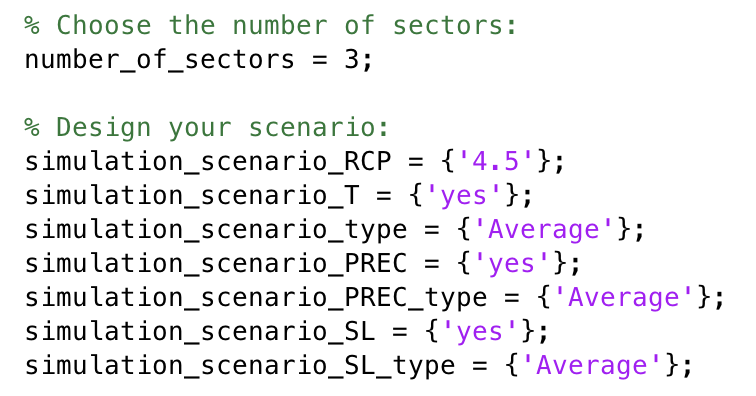
\includegraphics[width=7cm]{pictures/Scenario_Simulation/scensim05}}
		\end{figure}
		\item A descriptive name for the sceanrio will be assigned automatically 
	\end{itemize}
\end{frame}

%%%%%%%%%%%%%%%%%%%%%%%%%%%%%%%%%%%%%%%%%%%%%%%%%%%%%%%%

\end{document}